\large

\begin{minipage}{.43\columnwidth}
 \textbf{Optimizing the LP parameters}\\
 	The parameters; framelength $N$ and the overlap of frames $O$ are varied in order to determine the values for which the Prediction Gain (PG), is largest. The optimal coefficients are $N=1200$ and $O=1100$.
	\label{fig:HammingNOP10}
\end{minipage}% This must go next to `\end{minipage}`
\hspace{4mm}
\begin{minipage}[]{0.5\columnwidth}
	%	\includegraphics[width=\textwidth]{figures/HammingNOP10.pdf}
	% This file was created by matlab2tikz.
%
%The latest updates can be retrieved from
%  http://www.mathworks.com/matlabcentral/fileexchange/22022-matlab2tikz-matlab2tikz
%where you can also make suggestions and rate matlab2tikz.
%
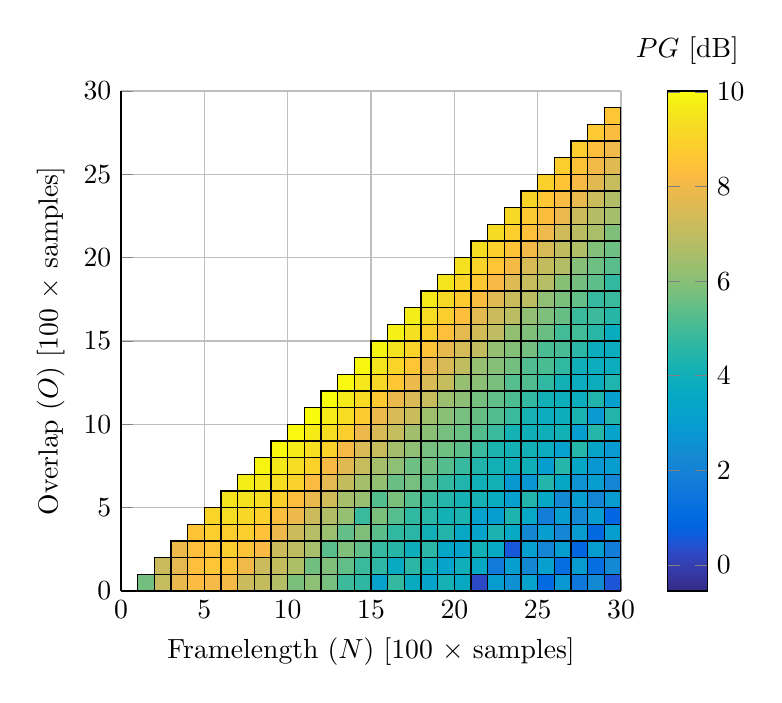
\begin{tikzpicture}


\begin{axis}[%
width=2.5in,
height=2.5in,
scale only axis,
point meta min=-0.551769511455843,
point meta max=10.0207598959184,
unbounded coords=jump,
xmin=0,
xmax=3000,
xlabel={Framelength ($N$) [100 $\times$ samples]},
xmajorgrids,
ymin=0,
ymax=3000,
ytick={0,500,...,3000},
yticklabels={0,5,...,30},
xtick={0,500,...,3000},
xticklabels={0,5,...,30},
ylabel={Overlap ($O$) [100 $\times$ samples]},
ymajorgrids,
axis background/.style={fill=white},
axis x line*=bottom,
axis y line*=left,
colormap={mymap}{[1pt] rgb(0pt)=(0.2081,0.1663,0.5292); rgb(1pt)=(0.211624,0.189781,0.577676); rgb(2pt)=(0.212252,0.213771,0.626971); rgb(3pt)=(0.2081,0.2386,0.677086); rgb(4pt)=(0.195905,0.264457,0.7279); rgb(5pt)=(0.170729,0.291938,0.779248); rgb(6pt)=(0.125271,0.324243,0.830271); rgb(7pt)=(0.0591333,0.359833,0.868333); rgb(8pt)=(0.0116952,0.38751,0.881957); rgb(9pt)=(0.00595714,0.408614,0.882843); rgb(10pt)=(0.0165143,0.4266,0.878633); rgb(11pt)=(0.0328524,0.443043,0.871957); rgb(12pt)=(0.0498143,0.458571,0.864057); rgb(13pt)=(0.0629333,0.47369,0.855438); rgb(14pt)=(0.0722667,0.488667,0.8467); rgb(15pt)=(0.0779429,0.503986,0.838371); rgb(16pt)=(0.0793476,0.520024,0.831181); rgb(17pt)=(0.0749429,0.537543,0.826271); rgb(18pt)=(0.0640571,0.556986,0.823957); rgb(19pt)=(0.0487714,0.577224,0.822829); rgb(20pt)=(0.0343429,0.596581,0.819852); rgb(21pt)=(0.0265,0.6137,0.8135); rgb(22pt)=(0.0238905,0.628662,0.803762); rgb(23pt)=(0.0230905,0.641786,0.791267); rgb(24pt)=(0.0227714,0.653486,0.776757); rgb(25pt)=(0.0266619,0.664195,0.760719); rgb(26pt)=(0.0383714,0.674271,0.743552); rgb(27pt)=(0.0589714,0.683757,0.725386); rgb(28pt)=(0.0843,0.692833,0.706167); rgb(29pt)=(0.113295,0.7015,0.685857); rgb(30pt)=(0.145271,0.709757,0.664629); rgb(31pt)=(0.180133,0.717657,0.642433); rgb(32pt)=(0.217829,0.725043,0.619262); rgb(33pt)=(0.258643,0.731714,0.595429); rgb(34pt)=(0.302171,0.737605,0.571186); rgb(35pt)=(0.348167,0.742433,0.547267); rgb(36pt)=(0.395257,0.7459,0.524443); rgb(37pt)=(0.44201,0.748081,0.503314); rgb(38pt)=(0.487124,0.749062,0.483976); rgb(39pt)=(0.530029,0.749114,0.466114); rgb(40pt)=(0.570857,0.748519,0.44939); rgb(41pt)=(0.609852,0.747314,0.433686); rgb(42pt)=(0.6473,0.7456,0.4188); rgb(43pt)=(0.683419,0.743476,0.404433); rgb(44pt)=(0.71841,0.741133,0.390476); rgb(45pt)=(0.752486,0.7384,0.376814); rgb(46pt)=(0.785843,0.735567,0.363271); rgb(47pt)=(0.818505,0.732733,0.34979); rgb(48pt)=(0.850657,0.7299,0.336029); rgb(49pt)=(0.882433,0.727433,0.3217); rgb(50pt)=(0.913933,0.725786,0.306276); rgb(51pt)=(0.944957,0.726114,0.288643); rgb(52pt)=(0.973895,0.731395,0.266648); rgb(53pt)=(0.993771,0.745457,0.240348); rgb(54pt)=(0.999043,0.765314,0.216414); rgb(55pt)=(0.995533,0.786057,0.196652); rgb(56pt)=(0.988,0.8066,0.179367); rgb(57pt)=(0.978857,0.827143,0.163314); rgb(58pt)=(0.9697,0.848138,0.147452); rgb(59pt)=(0.962586,0.870514,0.1309); rgb(60pt)=(0.958871,0.8949,0.113243); rgb(61pt)=(0.959824,0.921833,0.0948381); rgb(62pt)=(0.9661,0.951443,0.0755333); rgb(63pt)=(0.9763,0.9831,0.0538)},
colorbar,
colorbar style={title=$PG$ [dB]}
]%ylabel={PG}

\addplot[%
surf,
opacity = ceil(\pgfplotspointmetatransformed),
shader=flat corner,draw=black,colormap={mymap}{[1pt] rgb(0pt)=(0.2081,0.1663,0.5292); rgb(1pt)=(0.211624,0.189781,0.577676); rgb(2pt)=(0.212252,0.213771,0.626971); rgb(3pt)=(0.2081,0.2386,0.677086); rgb(4pt)=(0.195905,0.264457,0.7279); rgb(5pt)=(0.170729,0.291938,0.779248); rgb(6pt)=(0.125271,0.324243,0.830271); rgb(7pt)=(0.0591333,0.359833,0.868333); rgb(8pt)=(0.0116952,0.38751,0.881957); rgb(9pt)=(0.00595714,0.408614,0.882843); rgb(10pt)=(0.0165143,0.4266,0.878633); rgb(11pt)=(0.0328524,0.443043,0.871957); rgb(12pt)=(0.0498143,0.458571,0.864057); rgb(13pt)=(0.0629333,0.47369,0.855438); rgb(14pt)=(0.0722667,0.488667,0.8467); rgb(15pt)=(0.0779429,0.503986,0.838371); rgb(16pt)=(0.0793476,0.520024,0.831181); rgb(17pt)=(0.0749429,0.537543,0.826271); rgb(18pt)=(0.0640571,0.556986,0.823957); rgb(19pt)=(0.0487714,0.577224,0.822829); rgb(20pt)=(0.0343429,0.596581,0.819852); rgb(21pt)=(0.0265,0.6137,0.8135); rgb(22pt)=(0.0238905,0.628662,0.803762); rgb(23pt)=(0.0230905,0.641786,0.791267); rgb(24pt)=(0.0227714,0.653486,0.776757); rgb(25pt)=(0.0266619,0.664195,0.760719); rgb(26pt)=(0.0383714,0.674271,0.743552); rgb(27pt)=(0.0589714,0.683757,0.725386); rgb(28pt)=(0.0843,0.692833,0.706167); rgb(29pt)=(0.113295,0.7015,0.685857); rgb(30pt)=(0.145271,0.709757,0.664629); rgb(31pt)=(0.180133,0.717657,0.642433); rgb(32pt)=(0.217829,0.725043,0.619262); rgb(33pt)=(0.258643,0.731714,0.595429); rgb(34pt)=(0.302171,0.737605,0.571186); rgb(35pt)=(0.348167,0.742433,0.547267); rgb(36pt)=(0.395257,0.7459,0.524443); rgb(37pt)=(0.44201,0.748081,0.503314); rgb(38pt)=(0.487124,0.749062,0.483976); rgb(39pt)=(0.530029,0.749114,0.466114); rgb(40pt)=(0.570857,0.748519,0.44939); rgb(41pt)=(0.609852,0.747314,0.433686); rgb(42pt)=(0.6473,0.7456,0.4188); rgb(43pt)=(0.683419,0.743476,0.404433); rgb(44pt)=(0.71841,0.741133,0.390476); rgb(45pt)=(0.752486,0.7384,0.376814); rgb(46pt)=(0.785843,0.735567,0.363271); rgb(47pt)=(0.818505,0.732733,0.34979); rgb(48pt)=(0.850657,0.7299,0.336029); rgb(49pt)=(0.882433,0.727433,0.3217); rgb(50pt)=(0.913933,0.725786,0.306276); rgb(51pt)=(0.944957,0.726114,0.288643); rgb(52pt)=(0.973895,0.731395,0.266648); rgb(53pt)=(0.993771,0.745457,0.240348); rgb(54pt)=(0.999043,0.765314,0.216414); rgb(55pt)=(0.995533,0.786057,0.196652); rgb(56pt)=(0.988,0.8066,0.179367); rgb(57pt)=(0.978857,0.827143,0.163314); rgb(58pt)=(0.9697,0.848138,0.147452); rgb(59pt)=(0.962586,0.870514,0.1309); rgb(60pt)=(0.958871,0.8949,0.113243); rgb(61pt)=(0.959824,0.921833,0.0948381); rgb(62pt)=(0.9661,0.951443,0.0755333); rgb(63pt)=(0.9763,0.9831,0.0538)},mesh/rows=30]
table[row sep=crcr, point meta=\thisrow{c}] {%
%
x	y	c\\
100	0	5.6827458135075\\
100	100	nan\\
100	200	nan\\
100	300	nan\\
100	400	nan\\
100	500	nan\\
100	600	nan\\
100	700	nan\\
100	800	nan\\
100	900	nan\\
100	1000	nan\\
100	1100	nan\\
100	1200	nan\\
100	1300	nan\\
100	1400	nan\\
100	1500	nan\\
100	1600	nan\\
100	1700	nan\\
100	1800	nan\\
100	1900	nan\\
100	2000	nan\\
100	2100	nan\\
100	2200	nan\\
100	2300	nan\\
100	2400	nan\\
100	2500	nan\\
100	2600	nan\\
100	2700	nan\\
100	2800	nan\\
100	2900	nan\\
200	0	7.0790317182078\\
200	100	7.18389489543295\\
200	200	nan\\
200	300	nan\\
200	400	nan\\
200	500	nan\\
200	600	nan\\
200	700	nan\\
200	800	nan\\
200	900	nan\\
200	1000	nan\\
200	1100	nan\\
200	1200	nan\\
200	1300	nan\\
200	1400	nan\\
200	1500	nan\\
200	1600	nan\\
200	1700	nan\\
200	1800	nan\\
200	1900	nan\\
200	2000	nan\\
200	2100	nan\\
200	2200	nan\\
200	2300	nan\\
200	2400	nan\\
200	2500	nan\\
200	2600	nan\\
200	2700	nan\\
200	2800	nan\\
200	2900	nan\\
300	0	7.8278797182668\\
300	100	7.75061670667307\\
300	200	7.94964232573768\\
300	300	nan\\
300	400	nan\\
300	500	nan\\
300	600	nan\\
300	700	nan\\
300	800	nan\\
300	900	nan\\
300	1000	nan\\
300	1100	nan\\
300	1200	nan\\
300	1300	nan\\
300	1400	nan\\
300	1500	nan\\
300	1600	nan\\
300	1700	nan\\
300	1800	nan\\
300	1900	nan\\
300	2000	nan\\
300	2100	nan\\
300	2200	nan\\
300	2300	nan\\
300	2400	nan\\
300	2500	nan\\
300	2600	nan\\
300	2700	nan\\
300	2800	nan\\
300	2900	nan\\
400	0	8.25982045157361\\
400	100	8.37365829237133\\
400	200	8.38994845512447\\
400	300	8.53395155897113\\
400	400	nan\\
400	500	nan\\
400	600	nan\\
400	700	nan\\
400	800	nan\\
400	900	nan\\
400	1000	nan\\
400	1100	nan\\
400	1200	nan\\
400	1300	nan\\
400	1400	nan\\
400	1500	nan\\
400	1600	nan\\
400	1700	nan\\
400	1800	nan\\
400	1900	nan\\
400	2000	nan\\
400	2100	nan\\
400	2200	nan\\
400	2300	nan\\
400	2400	nan\\
400	2500	nan\\
400	2600	nan\\
400	2700	nan\\
400	2800	nan\\
400	2900	nan\\
500	0	8.09522110947221\\
500	100	8.58404936019439\\
500	200	8.52476852167647\\
500	300	8.85395289600773\\
500	400	9.03400135477561\\
500	500	nan\\
500	600	nan\\
500	700	nan\\
500	800	nan\\
500	900	nan\\
500	1000	nan\\
500	1100	nan\\
500	1200	nan\\
500	1300	nan\\
500	1400	nan\\
500	1500	nan\\
500	1600	nan\\
500	1700	nan\\
500	1800	nan\\
500	1900	nan\\
500	2000	nan\\
500	2100	nan\\
500	2200	nan\\
500	2300	nan\\
500	2400	nan\\
500	2500	nan\\
500	2600	nan\\
500	2700	nan\\
500	2800	nan\\
500	2900	nan\\
600	0	8.05650724153339\\
600	100	8.54693570913705\\
600	200	8.8377683265956\\
600	300	8.82559971223848\\
600	400	9.28658312212634\\
600	500	9.52161535433559\\
600	600	nan\\
600	700	nan\\
600	800	nan\\
600	900	nan\\
600	1000	nan\\
600	1100	nan\\
600	1200	nan\\
600	1300	nan\\
600	1400	nan\\
600	1500	nan\\
600	1600	nan\\
600	1700	nan\\
600	1800	nan\\
600	1900	nan\\
600	2000	nan\\
600	2100	nan\\
600	2200	nan\\
600	2300	nan\\
600	2400	nan\\
600	2500	nan\\
600	2600	nan\\
600	2700	nan\\
600	2800	nan\\
600	2900	nan\\
700	0	7.20736652003549\\
700	100	8.01860060821804\\
700	200	8.5092217869215\\
700	300	8.85498614721321\\
700	400	9.13100370114176\\
700	500	9.43150883603405\\
700	600	9.74782220562509\\
700	700	nan\\
700	800	nan\\
700	900	nan\\
700	1000	nan\\
700	1100	nan\\
700	1200	nan\\
700	1300	nan\\
700	1400	nan\\
700	1500	nan\\
700	1600	nan\\
700	1700	nan\\
700	1800	nan\\
700	1900	nan\\
700	2000	nan\\
700	2100	nan\\
700	2200	nan\\
700	2300	nan\\
700	2400	nan\\
700	2500	nan\\
700	2600	nan\\
700	2700	nan\\
700	2800	nan\\
700	2900	nan\\
800	0	7.06129617908756\\
800	100	7.21625389795336\\
800	200	8.17024678080842\\
800	300	8.4506398874489\\
800	400	8.92543148972206\\
800	500	9.31059383665309\\
800	600	9.57358732259701\\
800	700	9.88474425342921\\
800	800	nan\\
800	900	nan\\
800	1000	nan\\
800	1100	nan\\
800	1200	nan\\
800	1300	nan\\
800	1400	nan\\
800	1500	nan\\
800	1600	nan\\
800	1700	nan\\
800	1800	nan\\
800	1900	nan\\
800	2000	nan\\
800	2100	nan\\
800	2200	nan\\
800	2300	nan\\
800	2400	nan\\
800	2500	nan\\
800	2600	nan\\
800	2700	nan\\
800	2800	nan\\
800	2900	nan\\
900	0	6.7603240209297\\
900	100	7.07027516643772\\
900	200	7.21503157848168\\
900	300	7.91680228410601\\
900	400	8.33413384154289\\
900	500	8.91700110520262\\
900	600	9.33441266257382\\
900	700	9.61050000584357\\
900	800	9.96602273571317\\
900	900	nan\\
900	1000	nan\\
900	1100	nan\\
900	1200	nan\\
900	1300	nan\\
900	1400	nan\\
900	1500	nan\\
900	1600	nan\\
900	1700	nan\\
900	1800	nan\\
900	1900	nan\\
900	2000	nan\\
900	2100	nan\\
900	2200	nan\\
900	2300	nan\\
900	2400	nan\\
900	2500	nan\\
900	2600	nan\\
900	2700	nan\\
900	2800	nan\\
900	2900	nan\\
1000	0	5.79141266758575\\
1000	100	6.6583846543796\\
1000	200	6.96560213501504\\
1000	300	7.24068731658401\\
1000	400	7.9395591224285\\
1000	500	8.31867811054653\\
1000	600	8.9754932003346\\
1000	700	9.34845065231673\\
1000	800	9.67344129050852\\
1000	900	9.99470564606262\\
1000	1000	nan\\
1000	1100	nan\\
1000	1200	nan\\
1000	1300	nan\\
1000	1400	nan\\
1000	1500	nan\\
1000	1600	nan\\
1000	1700	nan\\
1000	1800	nan\\
1000	1900	nan\\
1000	2000	nan\\
1000	2100	nan\\
1000	2200	nan\\
1000	2300	nan\\
1000	2400	nan\\
1000	2500	nan\\
1000	2600	nan\\
1000	2700	nan\\
1000	2800	nan\\
1000	2900	nan\\
1100	0	6.08510006030311\\
1100	100	5.66131684642677\\
1100	200	6.52494101151453\\
1100	300	6.8154749961067\\
1100	400	7.2221683246724\\
1100	500	7.85272239575603\\
1100	600	8.25834444268623\\
1100	700	8.98246828788382\\
1100	800	9.38384280669374\\
1100	900	9.67888280713376\\
1100	1000	10.0207598959184\\
1100	1100	nan\\
1100	1200	nan\\
1100	1300	nan\\
1100	1400	nan\\
1100	1500	nan\\
1100	1600	nan\\
1100	1700	nan\\
1100	1800	nan\\
1100	1900	nan\\
1100	2000	nan\\
1100	2100	nan\\
1100	2200	nan\\
1100	2300	nan\\
1100	2400	nan\\
1100	2500	nan\\
1100	2600	nan\\
1100	2700	nan\\
1100	2800	nan\\
1100	2900	nan\\
1200	0	5.75236385929885\\
1200	100	5.8893978793085\\
1200	200	5.3233876826882\\
1200	300	6.30245671838949\\
1200	400	6.70416183583482\\
1200	500	7.29231639499116\\
1200	600	7.73083236703484\\
1200	700	8.13278866080154\\
1200	800	8.95016901139914\\
1200	900	9.3575654964583\\
1200	1000	9.69962351631871\\
1200	1100	10.018452727616\\
1200	1200	nan\\
1200	1300	nan\\
1200	1400	nan\\
1200	1500	nan\\
1200	1600	nan\\
1200	1700	nan\\
1200	1800	nan\\
1200	1900	nan\\
1200	2000	nan\\
1200	2100	nan\\
1200	2200	nan\\
1200	2300	nan\\
1200	2400	nan\\
1200	2500	nan\\
1200	2600	nan\\
1200	2700	nan\\
1200	2800	nan\\
1200	2900	nan\\
1300	0	4.8910628019805\\
1300	100	5.45072016874233\\
1300	200	5.86850066777867\\
1300	300	5.4597166268533\\
1300	400	6.21490882072339\\
1300	500	6.48849191466192\\
1300	600	7.05573401013256\\
1300	700	7.66870480877405\\
1300	800	8.12020714201073\\
1300	900	8.84241536316059\\
1300	1000	9.32521343768448\\
1300	1100	9.66682615033229\\
1300	1200	9.99393859933556\\
1300	1300	nan\\
1300	1400	nan\\
1300	1500	nan\\
1300	1600	nan\\
1300	1700	nan\\
1300	1800	nan\\
1300	1900	nan\\
1300	2000	nan\\
1300	2100	nan\\
1300	2200	nan\\
1300	2300	nan\\
1300	2400	nan\\
1300	2500	nan\\
1300	2600	nan\\
1300	2700	nan\\
1300	2800	nan\\
1300	2900	nan\\
1400	0	4.68328180207416\\
1400	100	4.87031890586883\\
1400	200	5.46124064783872\\
1400	300	5.87957713868692\\
1400	400	4.86401495955569\\
1400	500	6.26391766665361\\
1400	600	6.48566475687751\\
1400	700	7.13851035956643\\
1400	800	7.50027034876972\\
1400	900	7.94746340189027\\
1400	1000	8.77453134934714\\
1400	1100	9.23762319980819\\
1400	1200	9.58536439829166\\
1400	1300	9.93647418346277\\
1400	1400	nan\\
1400	1500	nan\\
1400	1600	nan\\
1400	1700	nan\\
1400	1800	nan\\
1400	1900	nan\\
1400	2000	nan\\
1400	2100	nan\\
1400	2200	nan\\
1400	2300	nan\\
1400	2400	nan\\
1400	2500	nan\\
1400	2600	nan\\
1400	2700	nan\\
1400	2800	nan\\
1400	2900	nan\\
1500	0	3.24765243794076\\
1500	100	4.65481232593174\\
1500	200	4.79830988957897\\
1500	300	5.35751567095906\\
1500	400	5.79287838471904\\
1500	500	5.25522140259071\\
1500	600	6.17072553135157\\
1500	700	6.48214041903959\\
1500	800	7.1345332299744\\
1500	900	7.48068047659614\\
1500	1000	7.89377405226484\\
1500	1100	8.70610504087698\\
1500	1200	9.16324372984275\\
1500	1300	9.52474035946379\\
1500	1400	9.86030813520319\\
1500	1500	nan\\
1500	1600	nan\\
1500	1700	nan\\
1500	1800	nan\\
1500	1900	nan\\
1500	2000	nan\\
1500	2100	nan\\
1500	2200	nan\\
1500	2300	nan\\
1500	2400	nan\\
1500	2500	nan\\
1500	2600	nan\\
1500	2700	nan\\
1500	2800	nan\\
1500	2900	nan\\
1600	0	4.75276003383697\\
1600	100	3.67495640572055\\
1600	200	4.52251715002299\\
1600	300	4.70771251796696\\
1600	400	5.26201893473007\\
1600	500	5.81200015855313\\
1600	600	5.54198269350814\\
1600	700	6.09112217072302\\
1600	800	6.43437379918348\\
1600	900	7.09943797512656\\
1600	1000	7.48241897845622\\
1600	1100	7.90693168041642\\
1600	1200	8.6380368658202\\
1600	1300	9.0916878406797\\
1600	1400	9.45586978035725\\
1600	1500	9.79114079162636\\
1600	1600	nan\\
1600	1700	nan\\
1600	1800	nan\\
1600	1900	nan\\
1600	2000	nan\\
1600	2100	nan\\
1600	2200	nan\\
1600	2300	nan\\
1600	2400	nan\\
1600	2500	nan\\
1600	2600	nan\\
1600	2700	nan\\
1600	2800	nan\\
1600	2900	nan\\
1700	0	3.71748664243527\\
1700	100	4.60591980476924\\
1700	200	3.91362630267876\\
1700	300	4.55847242510564\\
1700	400	4.70161157949911\\
1700	500	5.26688872672145\\
1700	600	5.74077415219596\\
1700	700	5.60918413969161\\
1700	800	6.12512258839059\\
1700	900	6.40152380276071\\
1700	1000	7.16577614393491\\
1700	1100	7.4954835376692\\
1700	1200	7.90408510720934\\
1700	1300	8.57357709454054\\
1700	1400	9.0277543415418\\
1700	1500	9.3764265164728\\
1700	1600	9.7243052974142\\
1700	1700	nan\\
1700	1800	nan\\
1700	1900	nan\\
1700	2000	nan\\
1700	2100	nan\\
1700	2200	nan\\
1700	2300	nan\\
1700	2400	nan\\
1700	2500	nan\\
1700	2600	nan\\
1700	2700	nan\\
1700	2800	nan\\
1700	2900	nan\\
1800	0	3.3177087556264\\
1800	100	4.01520154764494\\
1800	200	4.58897692120239\\
1800	300	4.05120880760072\\
1800	400	4.53307279512351\\
1800	500	4.80647025338146\\
1800	600	5.30764576164913\\
1800	700	5.66202006578872\\
1800	800	5.75312164595155\\
1800	900	6.04395256930141\\
1800	1000	6.3700405132766\\
1800	1100	7.14316992342896\\
1800	1200	7.48470310198768\\
1800	1300	7.87037714378024\\
1800	1400	8.48717243248572\\
1800	1500	8.92938209706209\\
1800	1600	9.3014704008889\\
1800	1700	9.64275886586559\\
1800	1800	nan\\
1800	1900	nan\\
1800	2000	nan\\
1800	2100	nan\\
1800	2200	nan\\
1800	2300	nan\\
1800	2400	nan\\
1800	2500	nan\\
1800	2600	nan\\
1800	2700	nan\\
1800	2800	nan\\
1800	2900	nan\\
1900	0	4.16438107268957\\
1900	100	3.30621453732177\\
1900	200	3.45177011062336\\
1900	300	4.41976545924296\\
1900	400	4.07826463673203\\
1900	500	4.47250181773447\\
1900	600	4.74401157157616\\
1900	700	5.27110068830706\\
1900	800	5.6301314654757\\
1900	900	5.74823980250472\\
1900	1000	6.03395598979113\\
1900	1100	6.3316791328726\\
1900	1200	7.11053211593739\\
1900	1300	7.45923534882344\\
1900	1400	7.81374082935247\\
1900	1500	8.40334989731675\\
1900	1600	8.81911874169977\\
1900	1700	9.19800880789435\\
1900	1800	9.54583520361966\\
1900	1900	nan\\
1900	2000	nan\\
1900	2100	nan\\
1900	2200	nan\\
1900	2300	nan\\
1900	2400	nan\\
1900	2500	nan\\
1900	2600	nan\\
1900	2700	nan\\
1900	2800	nan\\
1900	2900	nan\\
2000	0	3.63837130417713\\
2000	100	3.96838494244702\\
2000	200	3.28360542391229\\
2000	300	3.55278143786063\\
2000	400	4.26805123856089\\
2000	500	4.15389920807166\\
2000	600	4.39329679744196\\
2000	700	4.78828316129288\\
2000	800	5.37993737198608\\
2000	900	5.58147465390246\\
2000	1000	5.7286955025126\\
2000	1100	6.07285315548354\\
2000	1200	6.23857857671884\\
2000	1300	7.01013622331059\\
2000	1400	7.40631428562525\\
2000	1500	7.74343597295201\\
2000	1600	8.32757229622458\\
2000	1700	8.74188942454939\\
2000	1800	9.09209523315045\\
2000	1900	9.44134118935649\\
2000	2000	nan\\
2000	2100	nan\\
2000	2200	nan\\
2000	2300	nan\\
2000	2400	nan\\
2000	2500	nan\\
2000	2600	nan\\
2000	2700	nan\\
2000	2800	nan\\
2000	2900	nan\\
2100	0	0.264623542453294\\
2100	100	3.63488656288565\\
2100	200	4.08913120930422\\
2100	300	3.28220109142383\\
2100	400	3.18039510652367\\
2100	500	4.19474057968373\\
2100	600	4.0275612369305\\
2100	700	4.39427002201494\\
2100	800	4.86473111214704\\
2100	900	5.25381195203792\\
2100	1000	5.52645898428144\\
2100	1100	5.71270454803943\\
2100	1200	6.05580569501984\\
2100	1300	6.23707654312965\\
2100	1400	7.00000513992408\\
2100	1500	7.3381894461935\\
2100	1600	7.70510502361266\\
2100	1700	8.27878784954097\\
2100	1800	8.66979451640054\\
2100	1900	9.0155911617751\\
2100	2000	9.34506416881835\\
2100	2100	nan\\
2100	2200	nan\\
2100	2300	nan\\
2100	2400	nan\\
2100	2500	nan\\
2100	2600	nan\\
2100	2700	nan\\
2100	2800	nan\\
2100	2900	nan\\
2200	0	2.95170309874089\\
2200	100	1.73360893357364\\
2200	200	3.61323080676111\\
2200	300	4.28061341062458\\
2200	400	3.02458697343151\\
2200	500	3.75811713713825\\
2200	600	4.06218778116715\\
2200	700	4.05610248843421\\
2200	800	4.30007538322245\\
2200	900	4.85697872751457\\
2200	1000	5.22977855686604\\
2200	1100	5.42728488717261\\
2200	1200	5.7742976825497\\
2200	1300	5.9578809065615\\
2200	1400	6.20369481654021\\
2200	1500	6.97748546317166\\
2200	1600	7.25905430947499\\
2200	1700	7.63071051415358\\
2200	1800	8.17187520251639\\
2200	1900	8.56846748612261\\
2200	2000	8.92936194092831\\
2200	2100	9.25326090597395\\
2200	2200	nan\\
2200	2300	nan\\
2200	2400	nan\\
2200	2500	nan\\
2200	2600	nan\\
2200	2700	nan\\
2200	2800	nan\\
2200	2900	nan\\
2300	0	2.53293217519118\\
2300	100	3.00938026182184\\
2300	200	0.551769511455843\\
2300	300	3.60726664380354\\
2300	400	4.36229780994093\\
2300	500	3.08643225262487\\
2300	600	2.82564622459287\\
2300	700	3.98306729613317\\
2300	800	4.11490314132238\\
2300	900	4.13618785976634\\
2300	1000	4.86317380717345\\
2300	1100	5.16517700158233\\
2300	1200	5.26664183435126\\
2300	1300	5.69684803139814\\
2300	1400	5.95135216558113\\
2300	1500	6.16719875147937\\
2300	1600	6.89154945837155\\
2300	1700	7.18393537254356\\
2300	1800	7.60032386475286\\
2300	1900	8.1060139824226\\
2300	2000	8.49168618698787\\
2300	2100	8.84145695288964\\
2300	2200	9.16963549024874\\
2300	2300	nan\\
2300	2400	nan\\
2300	2500	nan\\
2300	2600	nan\\
2300	2700	nan\\
2300	2800	nan\\
2300	2900	nan\\
2400	0	3.23692740006642\\
2400	100	2.2228524336536\\
2400	200	3.08472299555247\\
2400	300	2.2240377386973\\
2400	400	3.53887086816519\\
2400	500	4.42615653537038\\
2400	600	2.75840359129067\\
2400	700	4.0107386280573\\
2400	800	4.05214769333313\\
2400	900	4.00914531419853\\
2400	1000	4.17937149969251\\
2400	1100	4.74117848303689\\
2400	1200	5.2085286363726\\
2400	1300	5.19304330014419\\
2400	1400	5.69847355162021\\
2400	1500	5.87188705075393\\
2400	1600	6.15489171474828\\
2400	1700	6.89765995399639\\
2400	1800	7.11879031436815\\
2400	1900	7.49046026449902\\
2400	2000	8.04502341053814\\
2400	2100	8.40465258616035\\
2400	2200	8.73328129071907\\
2400	2300	9.06128194950849\\
2400	2400	nan\\
2400	2500	nan\\
2400	2600	nan\\
2400	2700	nan\\
2400	2800	nan\\
2400	2900	nan\\
2500	0	1.05000257678802\\
2500	100	3.09955807465487\\
2500	200	2.13019145244393\\
2500	300	2.98129659738565\\
2500	400	1.80823551110839\\
2500	500	3.44295461285468\\
2500	600	4.45023506033534\\
2500	700	3.03486862485067\\
2500	800	3.799754032993\\
2500	900	3.97648541270297\\
2500	1000	3.83352254491892\\
2500	1100	4.04591105923088\\
2500	1200	4.69567516678935\\
2500	1300	5.11099504335296\\
2500	1400	5.09859465247581\\
2500	1500	5.57858218898721\\
2500	1600	5.8569467833986\\
2500	1700	6.10341874446816\\
2500	1800	6.81391868519097\\
2500	1900	7.03573319906174\\
2500	2000	7.42018466644079\\
2500	2100	7.9589647003702\\
2500	2200	8.29921705504155\\
2500	2300	8.63637971004693\\
2500	2400	8.96380635737141\\
2500	2500	nan\\
2500	2600	nan\\
2500	2700	nan\\
2500	2800	nan\\
2500	2900	nan\\
2600	0	2.80208415075651\\
2600	100	1.17194843956108\\
2600	200	2.96109260453396\\
2600	300	2.19270843592341\\
2600	400	3.0115728867441\\
2600	500	2.28393968299924\\
2600	600	3.47369768467374\\
2600	700	4.50853743880052\\
2600	800	3.15812371844604\\
2600	900	4.07856863803736\\
2600	1000	3.91468626002954\\
2600	1100	3.89808210094217\\
2600	1200	4.04567753651072\\
2600	1300	4.70566985097843\\
2600	1400	5.07194378908158\\
2600	1500	4.99752267777982\\
2600	1600	5.52550384847648\\
2600	1700	5.79174211203976\\
2600	1800	6.00046246850643\\
2600	1900	6.74511848933576\\
2600	2000	6.98699179435392\\
2600	2100	7.31013917497011\\
2600	2200	7.87653800818457\\
2600	2300	8.22494050640918\\
2600	2400	8.54322091765009\\
2600	2500	8.85820789226427\\
2600	2600	nan\\
2600	2700	nan\\
2600	2800	nan\\
2600	2900	nan\\
2700	0	1.58184394833386\\
2700	100	2.92525400331244\\
2700	200	0.887359676794604\\
2700	300	2.93101822389555\\
2700	400	2.30024404624266\\
2700	500	3.00032580576816\\
2700	600	2.58705024710389\\
2700	700	3.44496986930798\\
2700	800	4.4916042025927\\
2700	900	2.98522379998911\\
2700	1000	4.25749977657229\\
2700	1100	3.87067312264047\\
2700	1200	3.83784894949447\\
2700	1300	3.98929857887126\\
2700	1400	4.59197088590304\\
2700	1500	4.99312405800586\\
2700	1600	4.86180118194934\\
2700	1700	5.46261986535732\\
2700	1800	5.70973165052257\\
2700	1900	5.97276788996415\\
2700	2000	6.67403857872095\\
2700	2100	6.91286174850295\\
2700	2200	7.25280658811363\\
2700	2300	7.81626379934614\\
2700	2400	8.13648239969618\\
2700	2500	8.46913649633422\\
2700	2600	8.78457026475621\\
2700	2700	nan\\
2700	2800	nan\\
2700	2900	nan\\
2800	0	2.2987560540242\\
2800	100	1.19896433152671\\
2800	200	2.95163573066064\\
2800	300	0.973202079270705\\
2800	400	2.97370455963156\\
2800	500	2.12856324963795\\
2800	600	2.98222869928969\\
2800	700	2.77033362268512\\
2800	800	3.38784440474213\\
2800	900	4.50283031414694\\
2800	1000	2.86687295264398\\
2800	1100	4.3797702935594\\
2800	1200	3.86077604223459\\
2800	1300	3.88445747215116\\
2800	1400	3.88641891122799\\
2800	1500	4.54099461834347\\
2800	1600	4.89171252973565\\
2800	1700	4.80102017502878\\
2800	1800	5.38055416094404\\
2800	1900	5.62096395390293\\
2800	2000	5.9064550594499\\
2800	2100	6.57396144817971\\
2800	2200	6.77884258803287\\
2800	2300	7.20159987892983\\
2800	2400	7.70137646156138\\
2800	2500	8.02001565102648\\
2800	2600	8.3537017651593\\
2800	2700	8.6861911739627\\
2800	2800	nan\\
2800	2900	nan\\
2900	0	0.49312967237007\\
2900	100	2.25840014462245\\
2900	200	1.80380427347787\\
2900	300	3.03746280090745\\
2900	400	0.845717353642782\\
2900	500	2.91980222011896\\
2900	600	2.20120210963457\\
2900	700	2.99077861803715\\
2900	800	2.87641657842737\\
2900	900	3.26134076790394\\
2900	1000	4.42889490862495\\
2900	1100	3.07565824698724\\
2900	1200	4.36835391429797\\
2900	1300	3.8835622884345\\
2900	1400	3.84533451378335\\
2900	1500	3.78342493811934\\
2900	1600	4.5195926660129\\
2900	1700	4.84979739867748\\
2900	1800	4.72342685477777\\
2900	1900	5.32512315595608\\
2900	2000	5.60997138907586\\
2900	2100	5.87473951276466\\
2900	2200	6.48270953309765\\
2900	2300	6.71059287812374\\
2900	2400	7.1263819393935\\
2900	2500	7.63768597628047\\
2900	2600	7.95785638792816\\
2900	2700	8.27184455059282\\
2900	2800	8.58887864737359\\
2900	2900	nan\\
3000	0	-0.084166652386565\\
3000	100	0.658799202686103\\
3000	200	2.4286786445431\\
3000	300	2.00173215444182\\
3000	400	3.04605438638216\\
3000	500	0.804121831033953\\
3000	600	2.80060747061573\\
3000	700	2.10723369617921\\
3000	800	3.00606491677149\\
3000	900	2.9921027849289\\
3000	1000	3.2003941437714\\
3000	1100	4.47914328347861\\
3000	1200	3.09026222985996\\
3000	1300	4.40877799382241\\
3000	1400	3.86783693309201\\
3000	1500	3.82141825431614\\
3000	1600	3.75968653309083\\
3000	1700	4.42136187911435\\
3000	1800	4.73062760871956\\
3000	1900	4.65092537646692\\
3000	2000	5.26464935536502\\
3000	2100	5.53276290699877\\
3000	2200	5.79426518264794\\
3000	2300	6.43034113528171\\
3000	2400	6.61621727344431\\
3000	2500	6.98815251985862\\
3000	2600	7.51974760550906\\
3000	2700	7.84037752158828\\
3000	2800	8.1530922590658\\
3000	2900	8.49883156713133\\
};
\end{axis}
\end{tikzpicture}%
\end{minipage}

\vspace{4mm}
\begin{minipage}{.43\columnwidth}
	\textbf{System Delay Attenuation}\\
Without introduced system delay, prediction is unnecessary, as the FXLMS algorithm (\textcolor{MATLABblue}{---}) alone, will achieve infinite attenuation. For increasing system delay, a LP FXLMS (\textcolor{MATLABred}{---}) has an increased attenuation, of up to 40 dB for delays below 14 samples at 48 $k$Hz.

%	If no system delay is present no prediction is needed, because the FXLMS algorithm (\textcolor{MATLABblue}{---}) achieves infinite attenuation.
%	The attenuation of the non-predicting algorithm decreases with delay. The predicting algorithm (\textcolor{MATLABred}{---}) however attenuate speech by $\geq$ 40 dB for delays of up to 14 samples at 48 $k$Hz.
\end{minipage}% This must go next to `\end{minipage}`
\hspace{4mm}
\begin{minipage}{0.5\columnwidth}
	%\includegraphics[width=\textwidth]{figures/DelayRatio.pdf}
	% This file was created by matlab2tikz.
%
%The latest updates can be retrieved from
%  http://www.mathworks.com/matlabcentral/fileexchange/22022-matlab2tikz-matlab2tikz
%where you can also make suggestions and rate matlab2tikz.
%
\definecolor{mycolor1}{rgb}{0.00000,0.44700,0.74100}%
\definecolor{mycolor2}{rgb}{0.85000,0.32500,0.09800}%
%
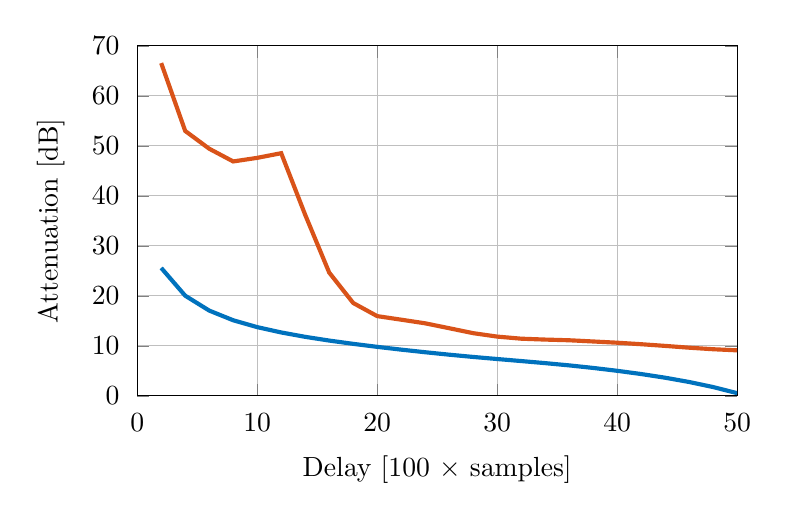
\begin{tikzpicture}

\begin{axis}[%
width=3in,
height=1.75in,
scale only axis,
xmin=0,
xmax=50,
xmajorgrids,
xlabel={Delay [100 $\times$ samples]},
ymin=0,
ymax=70,
ylabel style={yshift=0.3em},
xlabel style={yshift=-0.2em},
ytick={0,10,...,70},
ymajorgrids,
ylabel={Attenuation [dB]},
xticklabel shift={.1cm},
yticklabel shift={.1cm},
axis background/.style={fill=white}
]
\addplot [color=mycolor2,solid,line width=1.5pt,forget plot]
  table[row sep=crcr]{%
2	66.5420250310586\\
4	52.9717264302022\\
6	49.4175149424998\\
8	46.8717703569681\\
10	47.5886347675082\\
12	48.5221420089092\\
14	36.1913078215459\\
16	24.6480360536532\\
18	18.5625963047043\\
20	15.9345988709594\\
22	15.2225924490026\\
24	14.4941735350858\\
26	13.5145912190769\\
28	12.5242379572864\\
30	11.8400523957144\\
32	11.4203165228037\\
34	11.2428861871564\\
36	11.1050592495872\\
38	10.862823901561\\
40	10.6158645117455\\
42	10.3154480278615\\
44	9.97867799972119\\
46	9.61958031033587\\
48	9.31052791122033\\
50	9.08997582022533\\
};
\addplot [color=mycolor1,line width=1.5pt,solid,forget plot]
table[row sep=crcr]{%
	2	25.5751628128288\\
	4	20.0199680852144\\
	6	17.0442763613153\\
	8	15.1060127156582\\
	10	13.7310612019933\\
	12	12.6685774343164\\
	14	11.7903474171974\\
	16	11.0441690144364\\
	18	10.3883064900616\\
	20	9.78797702825996\\
	22	9.23075404560805\\
	24	8.7110676592604\\
	26	8.22176906503967\\
	28	7.77006791263877\\
	30	7.35426684398216\\
	32	6.94907270624338\\
	34	6.5323972441528\\
	36	6.08060777493347\\
	38	5.57101511941803\\
	40	4.99733350616245\\
	42	4.35167702165293\\
	44	3.61433096515684\\
	46	2.757705271237\\
	48	1.74470077738877\\
	50	0.5254168140125\\
};
\end{axis}
\end{tikzpicture}%
\end{minipage}
\vspace{4mm}

\begin{minipage}{.43\columnwidth}
\textbf{Frequency response comparison}\\
The frequency content of the FXLMS, (\textcolor{MATLABblue}{---}) is not changed much by the predictor (\textcolor{MATLABred}{---}), but the attenuation is increased by $\geq$ 15 dB. 
%	The attenuation of different frequencies for the FXLMS (\textcolor{MATLABblue}{---}) and the LP FXLMS  systems. The frequency content is not changed much by the predictor, 
\end{minipage}% This must go next to `\end{minipage}`
\hspace{4mm}
\begin{minipage}{0.5\columnwidth}
	%\includegraphics[width=\textwidth]{figures/ComparedConusmerHPOur.pdf}
	% This file was created by matlab2tikz.
%
%The latest updates can be retrieved from
%  http://www.mathworks.com/matlabcentral/fileexchange/22022-matlab2tikz-matlab2tikz
%where you can also make suggestions and rate matlab2tikz.
%

\definecolor{mycolor1}{rgb}{0.00000,0.44700,0.74100}%
\definecolor{mycolor2}{rgb}{0.85000,0.32500,0.09800}%
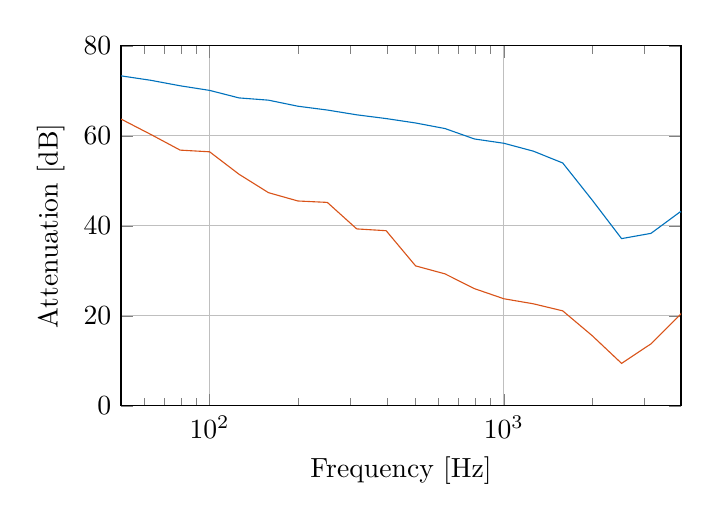
\begin{tikzpicture}

\begin{axis}[%
width=2.8in,
height=1.8in,
at={(1.011in,0.642in)},
scale only axis,
%scaled y ticks = false,
xmode=log,
xmin=50,
xmax=4000,
xlabel={Frequency [Hz]},
xmajorgrids,
ymin=0,
ymax=80,
ylabel={Attenuation [dB]},
ymajorgrids,
axis background/.style={fill=white},
title style={font=\bfseries},
%title={Comparison}
]
\addplot [color=mycolor1,solid,forget plot]
table[row sep=crcr]{%
	25.1188643150958	75.5409608467358\\
	31.6227766016838	75.9431721759286\\
	39.8107170553497	74.32582948051\\
	50.1187233627272	73.3120383257678\\
	63.0957344480193	72.3368435549144\\
	79.4328234724282	71.1136870555424\\
	100	70.0923048515607\\
	125.892541179417	68.4201295469469\\
	158.489319246111	67.9218525396411\\
	199.526231496888	66.5755639109352\\
	251.188643150958	65.7275603765609\\
	316.227766016838	64.6624593753836\\
	398.107170553497	63.8311887038426\\
	501.187233627272	62.8502765869508\\
	630.957344480193	61.610955662818\\
	794.328234724282	59.2960040541011\\
	1000	58.3414515564208\\
	1258.92541179417	56.5895979137366\\
	1584.89319246111	53.9618338486154\\
	1995.26231496888	45.7311859730353\\
	2511.88643150958	37.1520311323522\\
	3162.27766016838	38.3222077272126\\
	3981.07170553497	43.1414271757487\\
	5011.87233627272	37.7595452120207\\
	6309.57344480193	15.2746758953087\\
	7943.28234724281	9.59172966679038\\
	10000	19.8874971489198\\
	12589.2541179417	21.9362608444343\\
	15848.9319246111	26.8153847070164\\
	19952.6231496888	29.0588757352211\\
};
\addplot [color=mycolor2,solid,forget plot]
table[row sep=crcr]{%
	25.1188643150958	62.5141418875785\\
	31.6227766016838	61.3079673738348\\
	39.8107170553497	61.2318024067322\\
	50.1187233627272	63.6845315037753\\
	63.0957344480193	60.3097992334458\\
	79.4328234724282	56.8167941920522\\
	100	56.4448776773692\\
	125.892541179417	51.4548862652187\\
	158.489319246111	47.3641640933387\\
	199.526231496888	45.5160358037297\\
	251.188643150958	45.2005607673599\\
	316.227766016838	39.3099613460295\\
	398.107170553497	38.9102067178675\\
	501.187233627272	31.0916707503473\\
	630.957344480193	29.315552632249\\
	794.328234724282	26.0348627521026\\
	1000	23.7860460724777\\
	1258.92541179417	22.6691475414466\\
	1584.89319246111	21.0980560914196\\
	1995.26231496888	15.5926536914584\\
	2511.88643150958	9.42607294949861\\
	3162.27766016838	13.7675509770416\\
	3981.07170553497	20.2828603434003\\
	5011.87233627272	29.8933012343213\\
	6309.57344480193	16.830025003735\\
	7943.28234724281	14.3445849469403\\
	10000	30.2543194635927\\
	12589.2541179417	27.5461701991194\\
	15848.9319246111	25.8158178136092\\
	19952.6231496888	26.2476990595656\\
};
\end{axis}
\end{tikzpicture}%
\end{minipage}
